\documentclass[_main.tex]{subfiles}
 
\begin{document}

%\section{Basic principles}

\section*{The concept of a genomic transmission graph}

Imagine a directed acyclic graph in which the nodes represent hosts and edges represent vectors, as illustrated in figure \ref{fig:main_graph_1}.  The graph is plotted on an axis of time and we make the simplifying assumption that a host exists at a discrete point in time.  The directionality of the graph can be viewed in two ways.  When thinking about the transmission of parasites from host to host, we are moving forward in time so we follow the edges of the graph from left to right.  When thinking about the ancestry of a parasite, we are going back in time and therefore we follow the edges from right to left. 

%We do not show arrows on this graph but it is implicit that the edges are directed forwards in time to represent the transmission of parasites from host to host.  

\begin{figure}[h!]
\centering
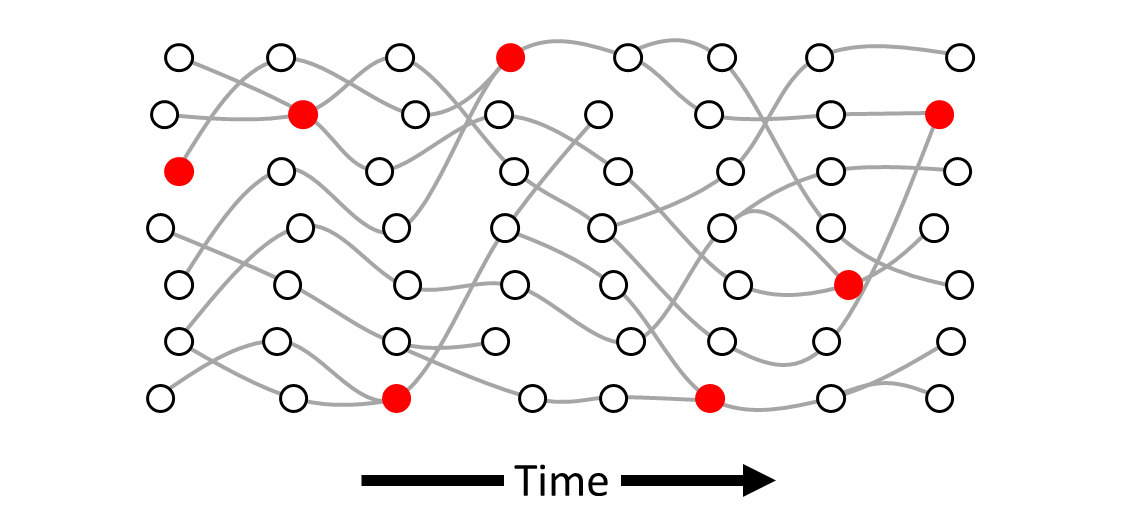
\includegraphics[width=10cm]{181001_tg_basic.png}
\caption{\textbf{An example of a transmission graph} representing all the transmission chains in some locality during some interval of time. Each node represents a host, i.e. a person that is carrying parasites and is capable of transmitting them to others.  Each edge represents a vector, i.e. a mosquito that transmits parasites from one host to another, and is therefore directed forwards in time. Red marks a node where transmission chains cross, representing a host that is superinfected.}
\label{fig:main_graph_1}
\end{figure}

If we pick any node and trace a path forward in time along the edges to other nodes, that is a \textit{transmission chain}. Some transmission chains terminate in a host that does not transmit to the next generation. Transmission chains can \textit{branch} when a host is the source of parasites for multiple other hosts.  Transmission chains can also \textit{cross} when a host acquires parasites from multiple sources, i.e when there is superinfection.   If transmission chains branch but do not cross then the graph will have a tree-like topology.  If there is both branching and crossing then the graph will have a reticulate structure as in figure \ref{fig:main_graph_1}.

%Parasites flow along transmission chains.  Hundreds of millions of people around the world are infected with \textit{P. falciparum}, and an infected person can carry billions of parasites.  However the majority of infected people do not pass on parasites to anyone else, and a vector transmits only a small number of parasites from one host to the next.  We refer to these as \textit{transmission bottlenecks} and they will be critical when we define the parameters of the transmission graph, because what interests us is how many parasite genomes are transmitted from one generation to the next.asite genomes are transmitted from one generation to the next.

%Parasite genomes undergo sexual recombination in the vector.  In a population without superinfection, recombination can only occur between parasites that are closely related as they must be descended from the same transmission chain.  Superinfection allows recombination between parasites that are genetically diverse due to the crossing of different transmission chains.

Parasites reproduce as they flow along transmission chains, and parasites that are flowing along the same transmission chain can genetically recombine with each other. We can use the transmission graph to account for recombination with the aid of three basic concepts:

\begin{itemize}[noitemsep]

\item A \textit{locus} is a specific location in the genome.  This could be anything from a single nucleotide position (which we call a \textit{point locus}) to a whole chromosome.

\item  An \textit{allele} is an instance of the parasite genome.  We usually speak of an allele with reference to a particular locus, in which case it means the DNA sequence of that locus in an individual parasite genome.

\item A \textit{lineage} is a path through the transmission graph that we define by taking an allele at a point locus and tracing its ancestry back in time through the generations. 

\end{itemize}

Our definition of a lineage specifically refers to a point locus because this is unaffected by recombination, so we can follow a lineage over many generations despite frequent recombination events.  Note that this definition differs from common usage, e.g. in the SARS-CoV-2 literature the term lineage refers to the viral genome as a whole.  A glossary of the terminology used in this paper is given at the end of this section.

An individual parasite could have many different lineages each following a unique path through the graph.  To understand how this is possible, imagine two point loci (A and B) in a parasite's genome.  If we trace the two corresponding lineages back in time, they are obliged to follow the same transmission chain until they reach a host that is superinfected, i.e. a node in the graph at which two transmission chains cross.  At that point their paths through the graph can diverge, because in the presence of recombination it is possible for locus A to be inherited from one of the transmission chains and locus B from the other (figure \ref{fig:superinfection1}).  This state of affairs means that times to coalescence can vary across the genome (figure \ref{fig:diff_lineage}) as we shall discuss in later sections.   

\begin{figure}[h!]
\centering
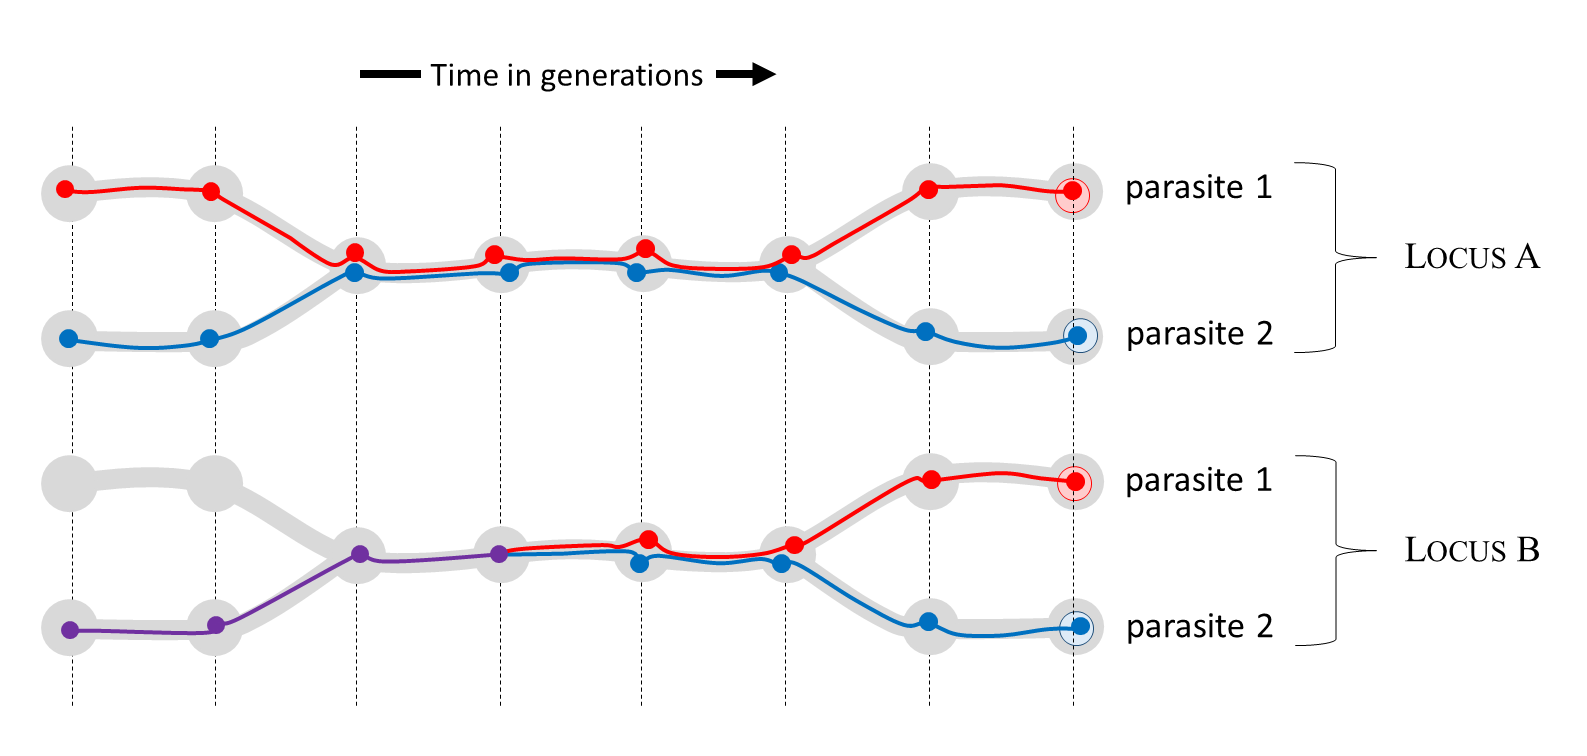
\includegraphics[width=10cm]{181003_lineages.png}
\caption{\textbf{Recombination causes coalescence times to vary across the genome}.  We sample two parasites (red and blue circles at far right) and trace their lineages back in time at two genomic loci, A and B.  Grey blobs represent hosts and broad grey lines represent transmission chains.  At locus A the red and blue lineages meet in the same transmission chain but separate again before coalescing.  At locus B the red and blue lineages meet in the same transmission chain and coalesce to form a single lineage marked in purple.}
\label{fig:diff_lineage}
\end{figure}

%A central theme of this paper will be to simulate the time to coalescence of two alleles at an arbitrary point locus, by following their lineages back in time until they coalesce in a common ancestral allele. Since recombination allows lineages of different loci to take different paths through the transmission graph,  it is evident that coalescence times must vary across the genome as illustrated in figure \ref{fig:diff_lineage}.  

%Each parasite carries one copy of the genome and, because we are primarily interested in how genome variation is transmitted through the generations, we call this the genomic transmission graph.

%We generally think of lineages and of coalescence from a historical perspective, i.e. going back in time, but if we are going forwards in time, coalescence implies that an allele has produced two copies of itself in the next generation.  

%We noted above that the combination of superinfection and recombination is problematic for phylodynamic analysis because it can cause different loci to have different phylogenies.  The transmission graph provides an alternative way to frame the problem, by allowing the lineages of different loci to diverge when transmission chains cross.

%refer to this as the genomic transmission graph as its primary purpose is to establish the quantitative relationship between transmission dynamics and genome variation.

These simple concepts suggest a logical framework for thinking about how genetic variation is related to transmission dynamics in a recombining parasite population.  Instead of attempting to construct a phylogenetic tree, we start by imagining a directed acyclic graph onto which we can map the lineages of different loci in the genome - we call this the genomic transmission graph.  This allows for superinfection and recombination because lineages at different loci can take different pathways through the graph.  We are left with two fundamental questions that are the main topic of this paper: what are the essential parameters of the genomic transmission graph and how are they mathematically related to parasite genetic variation?
  
%The problem then becomes how to infer essential parameters of the transmission graph from genetic features of the parasite population, and that is what we shall explore in the following sections.

\paragraph{Constructing an idealised genomic transmission graph} \label{idealised_tg}

A comprehensive model of parasite transmission dynamics would require consideration of many factors, e.g. hosts vary in their likelihood of getting infected, their duration of infection and their risk of infecting others, while vectors vary in their biting behaviour.  This could be achieved by embedding the genomic transmission graph within an agent-based epidemiological model but it would require the inclusion of a large number of parameters whose values we would need to guess.  As our aim is to estimate transmission parameters from genetic data, here we will construct an idealised model that makes a number of simplifying assumptions in order to minimise the number of parameters that need to be estimated.

When thinking about how genomes are transmitted through the generations, it is clear that some individuals have more progeny than others.  Hundreds of millions of people around the world are infected with \textit{P. falciparum} and an infected person can carry billions of parasites \cite{WHO2022}.  However the majority of infected people probably do not pass on parasites to anyone else, and a vector transmits only a small number of parasites from one host to the next \cite{Graumans2020}.  These population bottlenecks and \textit{transmission bottlenecks} are basic parameters of the genomic transmission graph.

Our idealised model imagines non-overlapping cycles of host to host transmission, and we refer to each cycle as a generation of the transmission graph (Figure \ref{fig:graph_2}).  We specify that: 

\begin{figure}[ht]
\centering
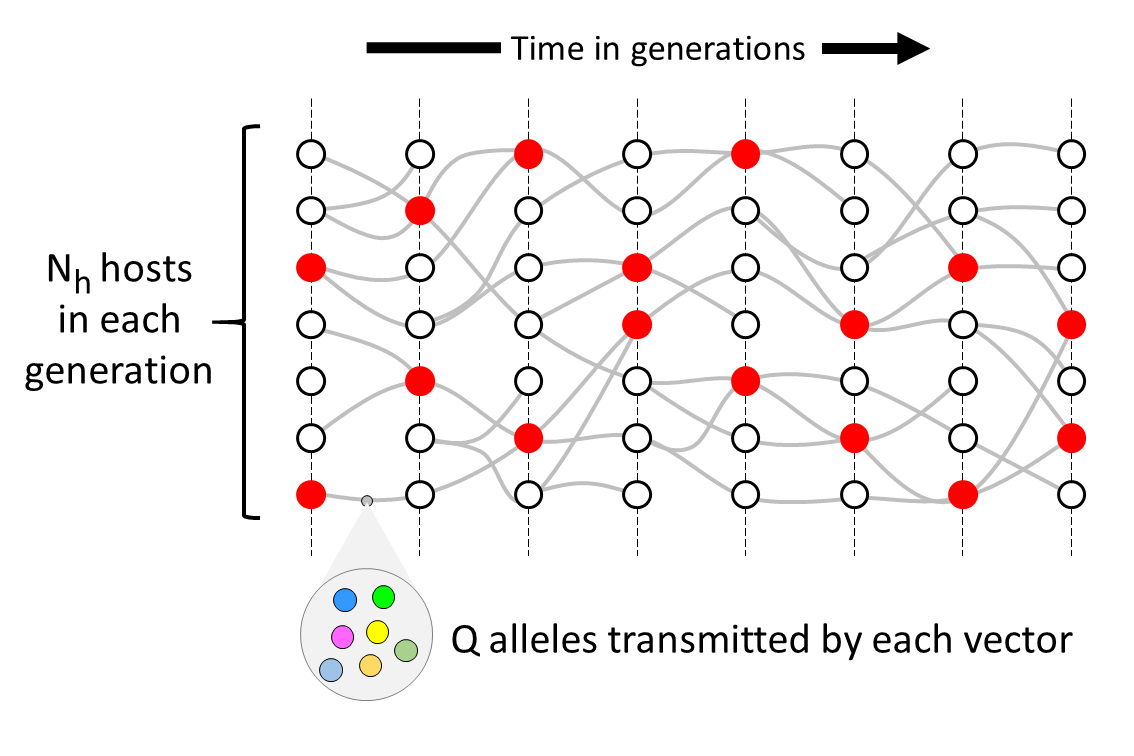
\includegraphics[width=10cm]{181002_tg_basic.png}
\caption{\textbf{An idealised model of the genomic transmission graph}.  We imagine that transmission occurs in non-overlapping generations.  In each generation there are $N_h$ hosts.  Each vector transmits $Q$ alleles to the recipient host.  $\chi$ is the crossing rate of transmission chains: this corresponds to the proportion of hosts that are superinfected from two sources, denoted in the figure by red nodes.}
\label{fig:graph_2}
\end{figure}

\begin{enumerate}

\item  There are $N_h$ hosts in each generation of the transmission graph: we refer to this as the \textbf{effective number of hosts}.  We can think of $N_h$ as the number of hosts that are in effect responsible for transmitting parasites from one generation to the next, which is likely to be much less than the total number of infected individuals, and represents a major population bottleneck.  The source of infection of a host is determined by random sampling with replacement from the $N_h$ hosts in the previous generation.

\item Each vector transmits $Q$ alleles to the recipient host: we call this the \textbf{quantum of transmission}.  We can think of $Q$ as the number of parasites that are inoculated by a mosquito into the host, but this is an over-simplification because $Q$ summarises a complex series of bottlenecks in host-vector and vector-host transmission occuring during one generation of the parasite life-cycle \cite{Chan2013,Graumans2020}.  The alleles transmitted to the recipient host are copied by random sampling with replacement from the alleles carried by the source host.

\item Each host has either one or two sources of infection in the previous generation, i.e. they are either superinfected or not.  The proportion of hosts that are superinfected is denoted $\chi$.  From the perspective of the genomic transmission graph, we refer to $\chi$ as the \textbf{crossing rate of transmission chains}. 

\end{enumerate}

This idealised model is obviously not an exact representation of the way things work in the real world.  For example, we specify that a host exists at a discrete point in time, so if the same person was infected at multiple time points, we would have to treat these as separate instances of being a host.  However our simplifying assumptions will be familiar to population geneticists as they are closely based on the Wright-Fisher model.  Indeed if $\chi=0$ and $Q = 1$ then the transmission graph is equivalent to a Wright-Fisher population of $N_h$ haploid individuals and, as will become clear in the next section, the Wright-Fisher model can be viewed as a special case of the idealised transmission graph.

\paragraph{Serial interval of transmission $\tau$.}  \label{main_serial_interval}  Let $\tau$ be the length of time corresponding to a generation of the transmission graph.  From a epidemiological perspective, this is equivalent to the mean serial interval between parasites entering one host and the next on a transmission chain.  Our model assumes that the serial interval is constant but in practice it ranges from approximately 6 weeks - the minimum time required for parasites to complete a full developmental cycle within the host and vector - to several years.  The mean serial interval probably depends many local factors, including the intensity and seasonality of malaria transmission. At this stage we do not need to specify the value of $\tau$ but this will be necessary later when we are estimating rates of mutation and recombination, and for the purpose of illustration we shall suppose that $\tau$ is approximately 3 months.

\paragraph{Relationship of $\chi$ to incidence of infection.} We have defined $\chi$ in terms of the transmission graph but what does it mean from an epidemiological perspective?  If $\chi = 0$ then each host on the transmission graph acquires infection from exactly one source.  We can therefore think of $\chi$ as the probability that a host acquires a new infection from another source during the same generation of the transmission graph.  If we make the simplifying assumption that this is approximately the same as the probability of any random individual acquiring a new infection, then the incidence of infection (i.e. the rate of infection per unit of time) is given by

\begin{equation}
\text{Incidence of infection} \approx \frac{\chi}{\tau}
\label{main:chi_tau} 
\end{equation}

This theoretical statement should be interpreted with caution as it is based on a number of simplifying assumptions, but it provides a practical motivation for estimating $\chi$ from genetic data, as a potential tool for detecting local fluctations in the incidence of infection when this is difficult to monitor by other means.

\end{document}